% ============================================================
% Ablation: model behavior under Baseline vs CASCADE
%
% Goal — two-layer behavioral characterisation:
%
% Layer 1 (within-model, Baseline): is the model conservative
%   (under-predicts the number of error categories per trace) or
%   aggressive (over-predicts), and does this prior bias correlate
%   with detection quality?
%
% Layer 2 (within-model, Baseline → CASCADE): does causal-graph
%   injection change the model's count behavior, and in which
%   direction? Is the behavioral shift consistent across splits?
%
% ------------------------------------------------------------
% Scoring methodology (for advisor review)
% ------------------------------------------------------------
%
% Per-trace count bias is:
%
%       s_t  =  log( (pred_t + 1) / (gold_t + 1) )
%
% where, for trace t:
%   gold_t  = number of *distinct* error categories present in the
%             human-annotated ground truth (i.e., set cardinality
%             after lower-casing and trimming category strings;
%             multiple span-level occurrences of the same
%             category count once).
%   pred_t  = number of *distinct* error categories the judge
%             predicted for the same trace, computed identically
%             from the model's parsed JSON output.
%
% Implementation: see figures/_plot_count_bias_likert.py
%   count_distinct_categories(errors)  — returns
%     |{ e.category.strip().lower() : e in errors if e.category }|
%   The two counts are then plugged into the log-ratio above.
%
% Design choices that may need discussion:
%
% (1) Category-level, not span-level. We collapse multiple
%     span-level error instances of the same category into a
%     single hit. Rationale: the +CG / +GI+SI prompt operates at
%     the category granularity (edges are A→B between categories),
%     and the W-F1 metric reported in the main results table is
%     also category-level (multi-label indicator over the 19/13
%     leaf categories). Span-level repetition is therefore not
%     part of the judge's category-detection task.
%
% (2) Laplace-style +1 smoothing in both numerator and denominator.
%     This handles three edge cases gracefully:
%       (a) gold = 0 (a trace with no annotated errors): without
%           smoothing, the ratio is undefined; with +1, the
%           score is +log(pred+1), monotone in over-prediction.
%       (b) pred = 0 (judge predicts no errors): symmetric
%           treatment via -log(gold+1).
%       (c) gold = pred (perfect count calibration): s = 0
%           regardless of the absolute count.
%     Trade-off: smoothing shrinks small-count differences toward
%     zero (e.g., 0-vs-1 maps to ±log 2 ≈ ±0.69, whereas 5-vs-6
%     maps to ≈ ±0.15). This is desirable for our use — large
%     absolute count differences should weigh more — but it does
%     mean low-recall traces dominate the tails of the CDF.
%
% (3) Log space (vs.\ raw pred − gold or pred/gold).
%     • symmetric around 0 (under- and over-prediction map to
%       equal-magnitude scores)
%     • additive interpretation: s = +1 means pred ≈ e × gold;
%       s = -1 means gold ≈ e × pred
%     • robust to outlier traces with very high gold counts that
%       would otherwise pull the linear difference distribution.
%     The chief alternative we considered, signed relative error
%     (pred - gold) / max(pred, gold), bounded to [-1, 1], gives a
%     bounded display but loses the additive interpretation that
%     makes the median meaningful as "typical multiplicative bias".
%
% (4) Per-trace summary statistic: median (not mean).
%     The CDFs are heavy-tailed (a handful of traces with very
%     high or low ratios) and the median is robust to those tails,
%     so it characterises the "typical" trace better than the
%     mean. We report the median directly in the per-panel
%     legend so a reader can compare cells arithmetically without
%     re-reading the curve.
%
% Score:  s = log( (pred + 1) / (gold + 1) )  per trace,
%         where pred / gold count distinct error categories.
%         s < 0  →  conservative (under-prediction)
%         s > 0  →  aggressive   (over-prediction)
%
% Source figure: figures/_plot_count_bias_cdf_cascade.{py,png}
%   Generator:   python figures/_plot_count_bias_cdf_cascade.py
%                  (default --method-pair Baseline,+GI+SI)
%   Variants:    --method-pair Baseline,+CG    → ablate one-pass +CG
%                --method-pair +CG,+GI+SI      → contrast injection style
% ============================================================

\begin{figure*}[t]
  \centering
  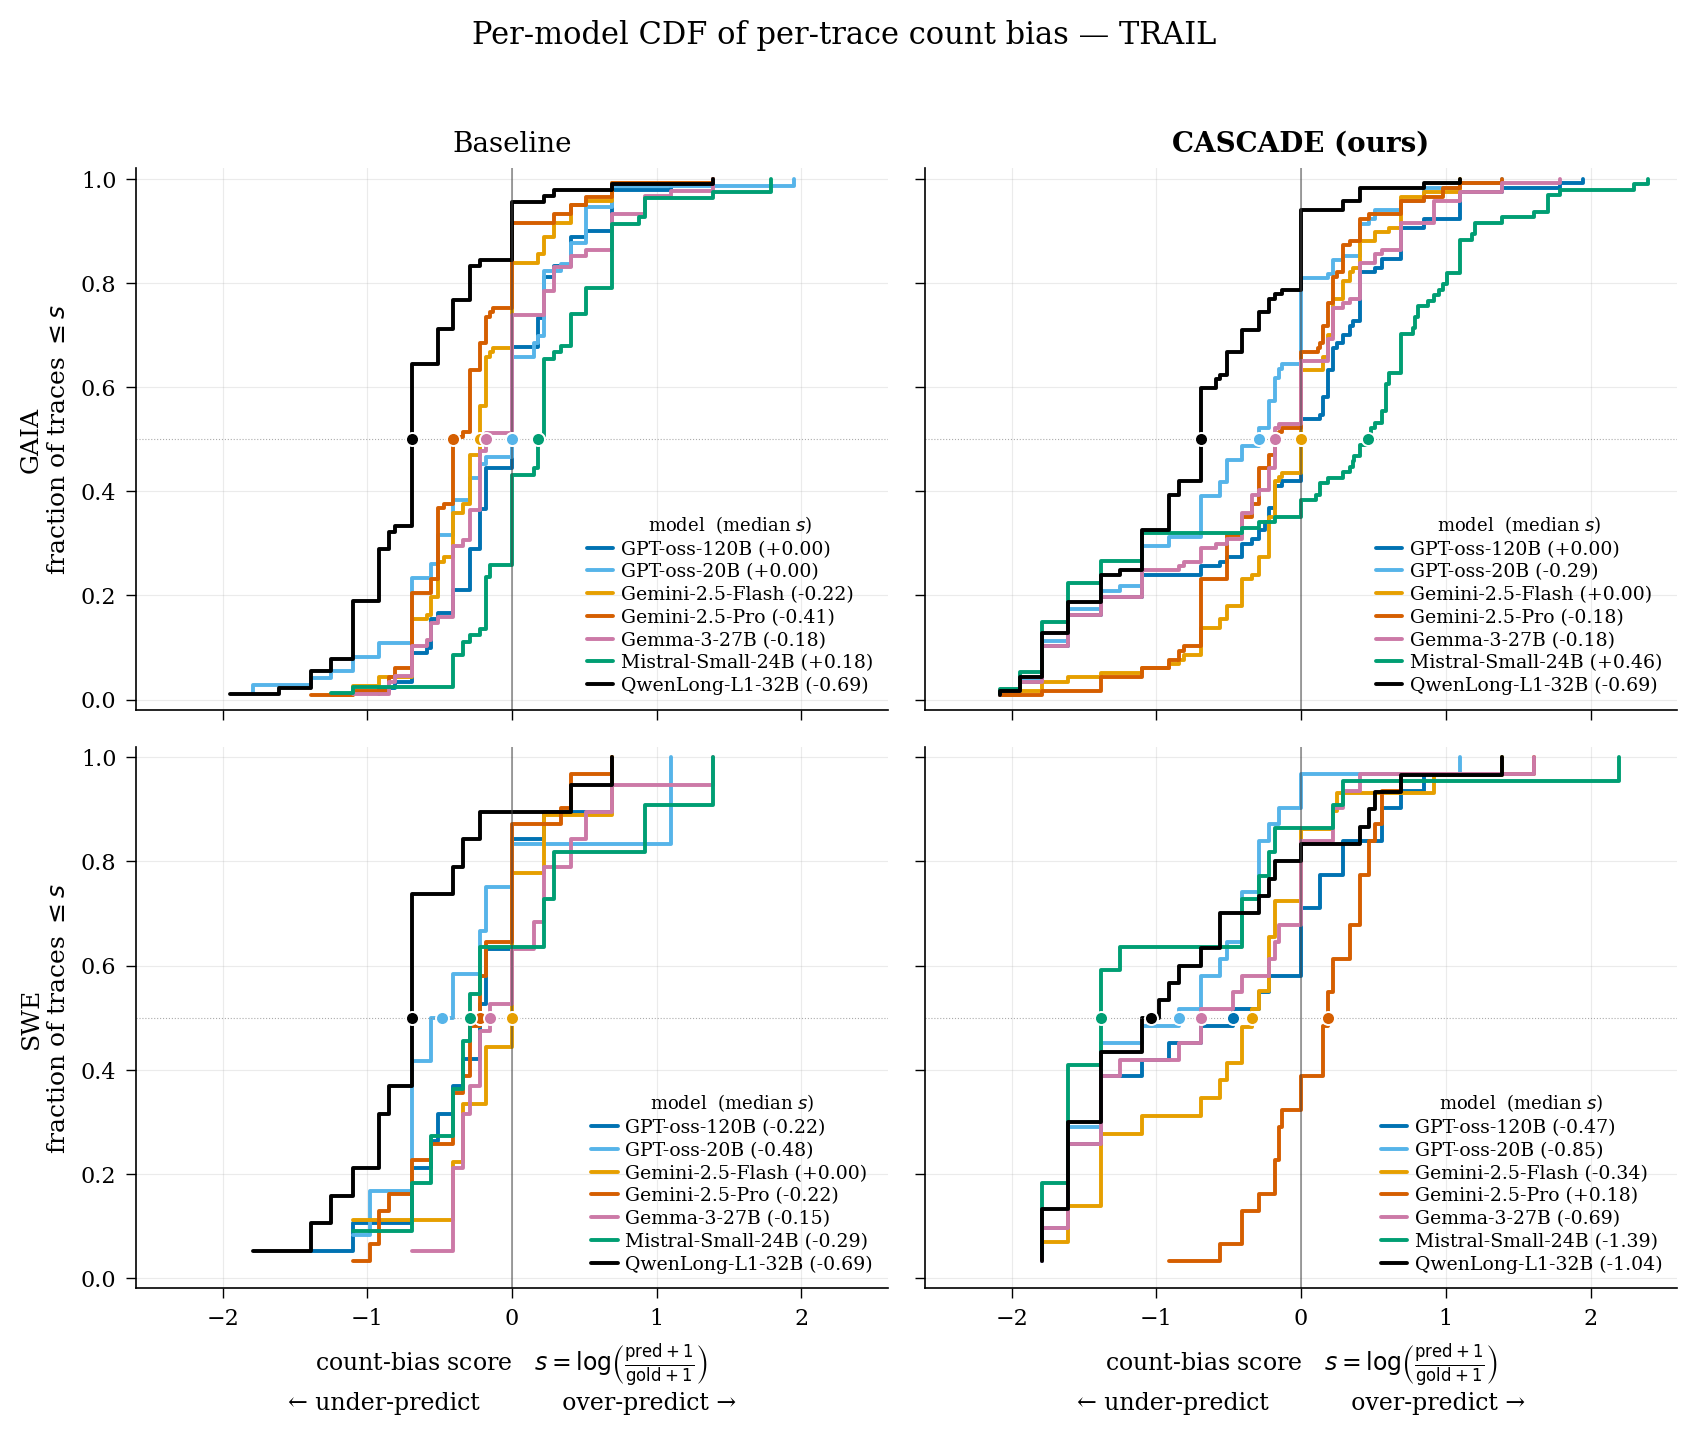
\includegraphics[width=0.95\linewidth]{figures/_plot_count_bias_cdf_baseline-cascade.png}
  \caption{%
    \textbf{Per-trace count bias under Baseline and CASCADE.}
    Each panel shows the cumulative distribution of the per-trace
    log-ratio
    $s = \log\!\bigl((\textit{pred} + 1)/(\textit{gold} + 1)\bigr)$,
    where \textit{pred} (resp.\ \textit{gold}) is the number of
    distinct error categories predicted (resp.\ annotated) for that
    trace. $s<0$ marks conservative (under-predicting) behavior;
    $s>0$ marks aggressive (over-predicting) behavior; the marker
    on each curve at $y{=}0.5$ is the model's median per-trace bias.
    Rows: TRAIL split (GAIA-dedup, SWE-Bench-dedup); columns:
    method (Baseline vs CASCADE, our two-pass dynamic graph
    injection corresponding to \texttt{+GI+SI} elsewhere in the
    paper). The signed value in each legend entry is the model's
    median $s$ on that (split, method) cell. Reading left-to-right
    within a row reveals whether causal-graph injection
    \emph{calibrates} the model's count (median moves toward zero),
    \emph{amplifies} its prior tendency (median moves further from
    zero in the same direction), or \emph{flips} the regime
    (median changes sign).%
  }
  \label{fig:ablation_behavior}
\end{figure*}


% ---------- Body text ----------

\paragraph{Layer 1: Baseline count behavior is split- and model-specific.}
We measure each model's per-trace count bias as
$s = \log((\text{pred}+1)/(\text{gold}+1))$ and read its median across
traces as a behavioral prior. Under the no-graph Baseline
(left columns of Fig.~\ref{fig:ablation_behavior}), most models on
\textbf{GAIA-dedup} are conservative — Gemini-2.5-Flash
($\tilde s {=} -0.22$), Gemini-2.5-Pro ($-0.41$), Gemma-3-27B
($-0.18$), and QwenLong-L1-32B ($-0.69$) all sit left of the zero
line; the two GPT-oss models are near-calibrated ($\tilde s {\approx} 0$);
Mistral-Small-24B is the sole over-predictor ($+0.18$). On
\textbf{SWE-Bench-dedup} the spread collapses: six of seven models
under-predict (Mistral $-0.29$, Gemini-Pro $-0.22$, GPT-oss-20B
$-0.48$, QwenLong $-0.69$, etc.), with Gemini-Flash the lone
near-calibrated case. The behavioral prior is therefore not a
fixed model property but a (model, dataset) interaction:
the same Mistral that over-predicts on GAIA under-predicts on SWE.
Mapping this onto detection quality, the strongest conservative
priors (QwenLong, Gemini-Pro on GAIA; Mistral, Gemma on SWE)
correspond to the lowest baseline W-F1 numbers in
Table~\ref{tab:main_results}, consistent with the intuition that
silent under-prediction caps recall before any graph guidance is
even introduced.

\paragraph{Layer 2: CASCADE shifts behavior, but the direction is split-dependent.}
Reading each row of Fig.~\ref{fig:ablation_behavior} left-to-right
(Baseline $\to$ CASCADE) reveals three qualitatively different
behavioral responses to causal-graph injection, and which response
fires depends largely on the split. On \textbf{GAIA-dedup} the
shifts are small and idiosyncratic: the median bias barely moves
for four of seven models ($|\Delta\tilde s|{\leq}0.05$);
Gemini-2.5-Flash and Pro are pulled towards calibration
($-0.22 \to 0.00$ and $-0.41 \to -0.18$); Mistral, already
aggressive at Baseline, is amplified further
($+0.18 \to +0.46$); GPT-oss-20B drifts from near-calibrated to
mildly conservative ($0.00 \to -0.29$). On
\textbf{SWE-Bench-dedup} the shift is large and uniformly directed:
six of seven models become \emph{more} conservative under CASCADE,
with Mistral undergoing the largest move
($-0.29 \to -1.39$, $\Delta\tilde s = -1.10$),
followed by Gemma ($-0.15 \to -0.69$), Gemini-Flash
($+0.00 \to -0.34$), GPT-oss-20B ($-0.48 \to -0.85$),
QwenLong ($-0.69 \to -1.04$), and GPT-oss-120B ($-0.22 \to -0.47$).
The lone exception is Gemini-2.5-Pro, which flips sign
($-0.22 \to +0.18$).
A natural hypothesis is that this asymmetry traces to the
ground-truth label structure, but the two splits in fact have the
same median number of distinct error categories per trace ($\sim$4
on both); what differs is the \emph{within-trace repetition} of
those categories — SWE traces average $8.3$ error spans across
$4.0$ distinct labels (${\sim}2.1$ instances per category) versus
GAIA's $5.0$ spans across $3.7$ labels (${\sim}1.4$ per category).
We therefore do not attribute the SWE-side conservativeness shift
to a missing-target story; possible mechanisms include (i) the
SWE corpus being small ($N{=}31$ vs.\ $117$), which amplifies
trace-level variance, (ii) longer per-trace context on SWE
diluting the graph block's relative weight, and (iii) a domain
mismatch in which the validated causal edges (extracted from
both splits jointly) align less tightly with the repetitive
code-edit / test-rerun error patterns that dominate SWE traces.
We flag this as a real behavioral phenomenon worth further
investigation, and discuss it as a limitation in
Sec.~\ref{sec:limitations}.

\paragraph{Implications for our method's design.}
The two-layer picture argues that calibration is not a single-axis
``the model under- or over-predicts'' property and that graph
guidance should not be evaluated solely by aggregate
W-F1/Loc/Joint. Two consequences for CASCADE: (i) the gains it
yields on aggregate metrics may partially come from \emph{absorbing}
a model's prior conservativeness rather than overcoming it,
particularly on SWE where the graph's net effect is to push
predictions \emph{further} into under-prediction; (ii) for any
model whose Baseline median already sits left of zero (which is
most open-source models on both splits in our panel), a more
calibration-aware graph prompt — for instance, suggesting both
``check for $B$'' and ``re-verify $A$ was actually an error'' —
might recover the recall that the current asymmetric
\emph{``look for more downstream errors''} formulation leaves
behind.

% Reproduce: python figures/_plot_count_bias_cdf_cascade.py
% Variants for appendix:
%   python figures/_plot_count_bias_cdf_cascade.py --method-pair Baseline,+CG
%   python figures/_plot_count_bias_cdf_cascade.py --method-pair +CG,+GI+SI
